\documentclass[final]{beamer}

\usepackage[scale=1.24]{beamerposter} % Use the beamerposter package for laying out the poster
\usepackage{csquotes}
\usepackage[american]{babel}
\usepackage[style=apa]{biblatex}
\usetheme{confposter} % Use the confposter theme supplied with this template
\setbeamercolor{block title}{fg=ngreen,bg=white} % Colors of the block titles
\setbeamercolor{block body}{fg=black,bg=white} % Colors of the body of blocks
\setbeamercolor{block alerted title}{fg=white,bg=dblue!70} % Colors of the highlighted block titles
\setbeamercolor{block alerted body}{fg=black,bg=dblue!10} % Colors of the body of highlighted blocks
% Many more colors are available for use in beamerthemeconfposter.sty
\usepackage{graphicx}
\graphicspath{{../results/graphs/pub/}}
\DeclareGraphicsExtensions{.pdf,.eps,.jpg}
\DeclareLanguageMapping{american}{american-apa}
\bibliography{stata2018}
%%%%%%%%%%%%%%%%%%%%%%%%%%%%%%%%%%%%%%%%%
% Jacobs Landscape Poster
% LaTeX Template
% Version 1.0 (29/03/13)
%
% Created by:
% Computational Physics and Biophysics Group, Jacobs University
% https://teamwork.jacobs-university.de:8443/confluence/display/CoPandBiG/LaTeX+Poster
% 
% Further modified by:
% Nathaniel Johnston (nathaniel@njohnston.ca)
%
% This template has been downloaded from:
% http://www.LaTeXTemplates.com
%
% License:
% CC BY-NC-SA 3.0 (http://creativecommons.org/licenses/by-nc-sa/3.0/)
%
%%%%%%%%%%%%%%%%%%%%%%%%%%%%%%%%%%%%%%%%%

%----------------------------------------------------------------------------------------
%	PACKAGES AND OTHER DOCUMENT CONFIGURATIONS
%----------------------------------------------------------------------------------------


%-----------------------------------------------------------
% Define the column widths and overall poster size
% To set effective sepwid, onecolwid and twocolwid values, first choose how many columns you want and how much separation you want between columns
% In this template, the separation width chosen is 0.024 of the paper width and a 4-column layout
% onecolwid should therefore be (1-(# of columns+1)*sepwid)/# of columns e.g. (1-(4+1)*0.024)/4 = 0.22
% Set twocolwid to be (2*onecolwid)+sepwid = 0.464
% Set threecolwid to be (3*onecolwid)+2*sepwid = 0.708

\newlength{\sepwid}
\newlength{\onecolwid}
\newlength{\twocolwid}
\newlength{\threecolwid}
\setlength{\paperwidth}{48in} % A0 width: 46.8in
\setlength{\paperheight}{36in} % A0 height: 33.1in
\setlength{\sepwid}{0.024\paperwidth} % Separation width (white space) between columns
\setlength{\onecolwid}{0.22\paperwidth} % Width of one column
\setlength{\twocolwid}{0.464\paperwidth} % Width of two columns
\setlength{\threecolwid}{0.708\paperwidth} % Width of three columns
\setlength{\topmargin}{-0.5in} % Reduce the top margin size
%-----------------------------------------------------------


\usepackage{booktabs} % Top and bottom rules for tables

%----------------------------------------------------------------------------------------
%	TITLE SECTION 
%----------------------------------------------------------------------------------------

\title{Exploring Legislative Cosponsorship Networks in Stata with \texttt{nwcommands}} % Poster title

\author{Roxana Del Campo \inst{1} \and Billy Buchanan \inst{2}} % Author(s)

\institute{\inst{1} University of Washington, College of Education \inst{2} PACES Consulting} % Institution(s)

%----------------------------------------------------------------------------------------

\begin{document}
	\addtobeamertemplate{block end}{}{\vspace*{2ex}} % White space under blocks
	\addtobeamertemplate{block alerted end}{}{\vspace*{2ex}} % White space under highlighted (alert) blocks
	\setlength{\belowcaptionskip}{2ex} % White space under figures
	\setlength\belowdisplayshortskip{2ex} % White space under equations
	% The whole poster is enclosed in one beamer frame
	\begin{frame}[t] 
		% The whole poster consists of three major columns, the second of which is 
		% split into two columns twice - the [t] option aligns each column's content to the top
		\begin{columns}[t] 
			% Empty spacer column
			\begin{column}{\sepwid}\end{column} 
				
			% The first column
			\begin{column}{\onecolwid} 
				\begin{figure}
					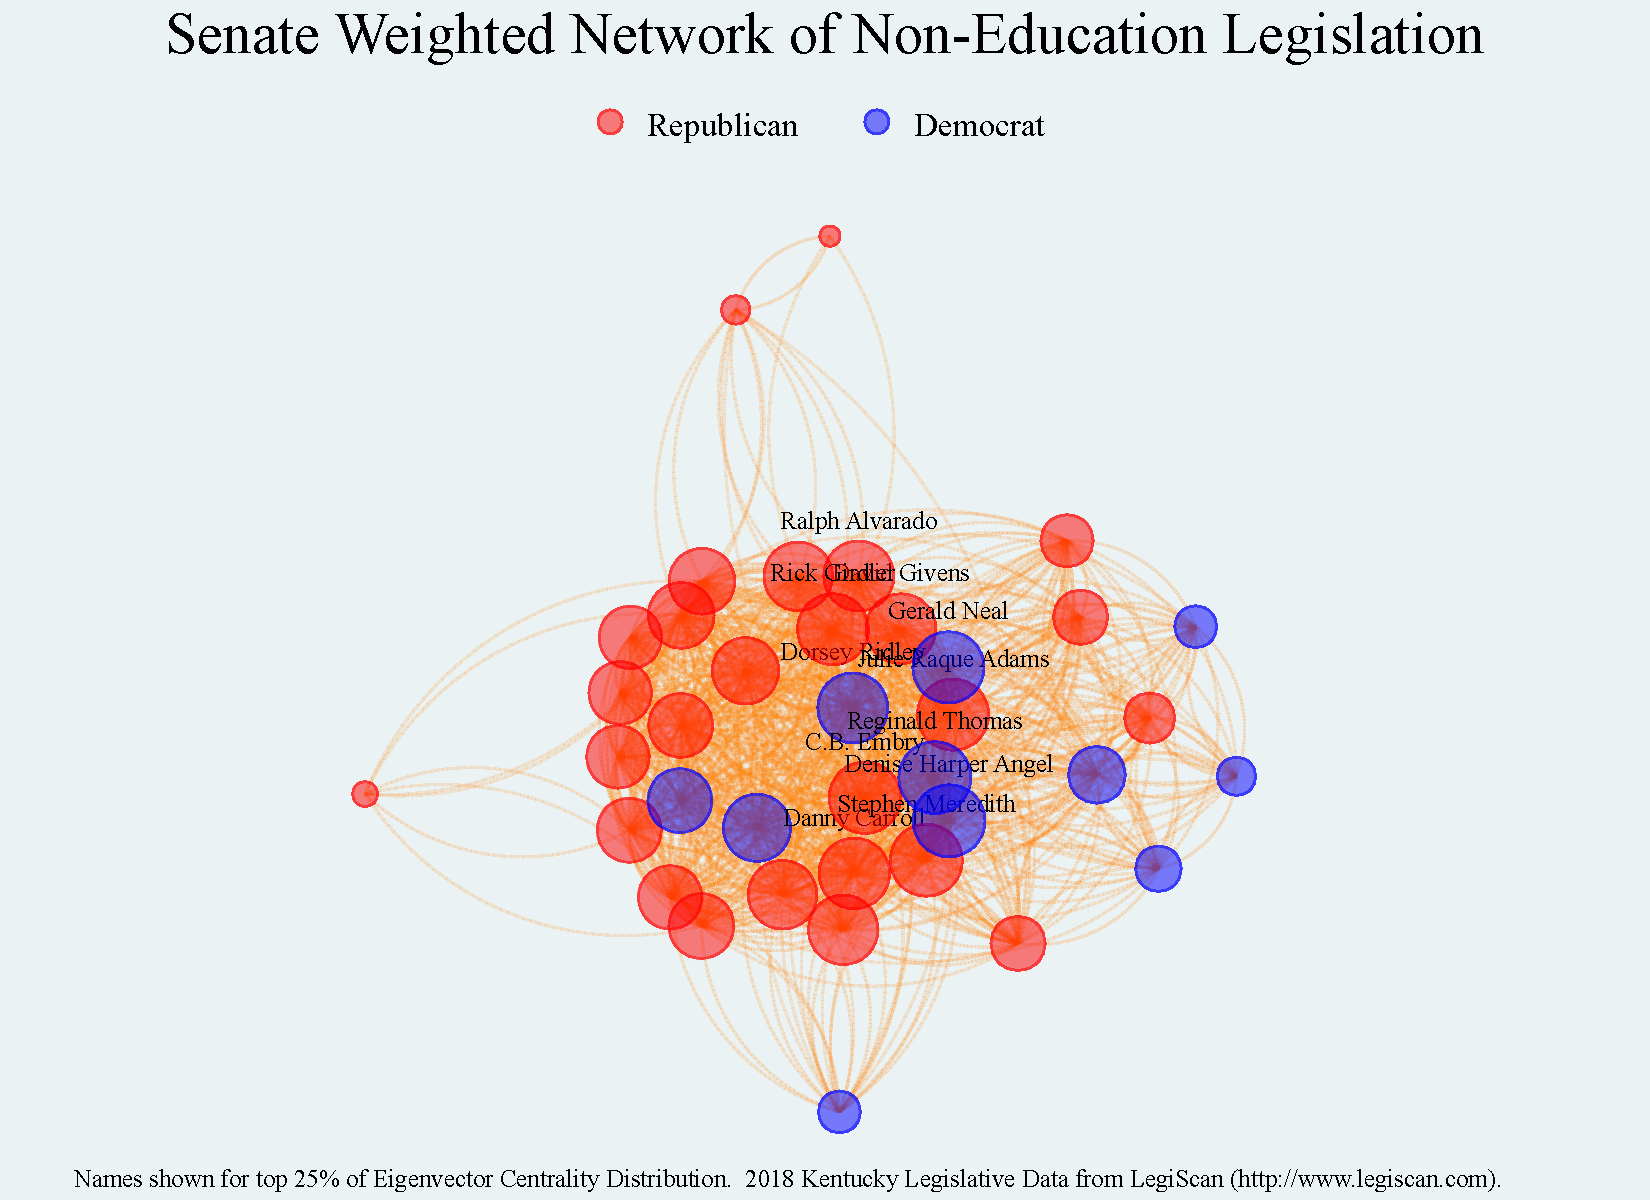
\includegraphics[scale=0.95]{senatenonedwgt-graph.pdf}
					\caption{Senate NECN \label{senatenoned}}
				\end{figure}
				%----------------------------------------------------------------------------------------
				%	OBJECTIVES
				%----------------------------------------------------------------------------------------
				\begin{block}{Goals}
					\begin{enumerate}
						\item{Do the cosponsorship networks vary between education and non-education legislation?} 
					   \item{Are legislative leaders highly influential in the context of legislation co-sponsorship?}
					   \item{Do the most influential legislators vary between education and non-education cosponsorship networks?}
					\end{enumerate}
				\end{block}
				%----------------------------------------------------------------------------------------
				%	INTRODUCTION
				%----------------------------------------------------------------------------------------
				\begin{block}{Introduction}
					Kentucky legislature is currently in the process of passing legislations regarding teacher 
					pension and educational public spending reform.   Through studying Kentucky's legislature 
					cosponsorship network, we aim to determine which legislators have a tendency of cosponsoring 
					educational legislature.  Data for legislative cosponsorship network has been used to identify 
					influential legislators \parencite{fowler2006}.  Defining strong networks of legislators can assist 
					groups lobbing for particular policies.  Examining the relationship between lobbyist and 
					legislators, \textcite{kroger2009} found common donors between legislators that have more agreements 
					in the legislative bill voting records.
				\end{block}
				\begin{block}{Study Sample}
					Our sample of legislators and bills is summarized below, \ref{sample}.  Data were obtained to define
					Non-Education Cosponsorship Networks (NECN) and Education Cosponsorship Networks (ECN).
					
					\begin{table}
						\caption{\textit{Distribution of Legislators and Bills Across Chambers and Party Lines.} \label{sample}}
						\begin{tabular}{l l l || l l}
							\toprule
							\textbf{Chamber} & \textbf{Party} & \textbf{Legislators} & \textbf{Bill Type} & \textbf{Bills} \\
							\midrule
							Senate & Democrat & 11 & Education & 45 \\
							Senate & Republican & 27 & Non-Education & 243 \\
							House & Democrat & 37 & Education & 45 \\
							House & Republican & 63 & Non-Education & 560 \\
							\bottomrule
						\end{tabular}
					\end{table}
										
				\end{block}
			\end{column} % End of the first column

			\begin{column}{\sepwid}\end{column} % Empty spacer column
			
			\begin{column}{\twocolwid} % Begin a column which is two columns wide (column 2)
				\begin{columns}[t,totalwidth=\twocolwid] % Split up the two columns wide column
					\begin{column}{\onecolwid}\vspace{-.6in} % The first column within column 2 (column 2.1)
						\begin{figure}
							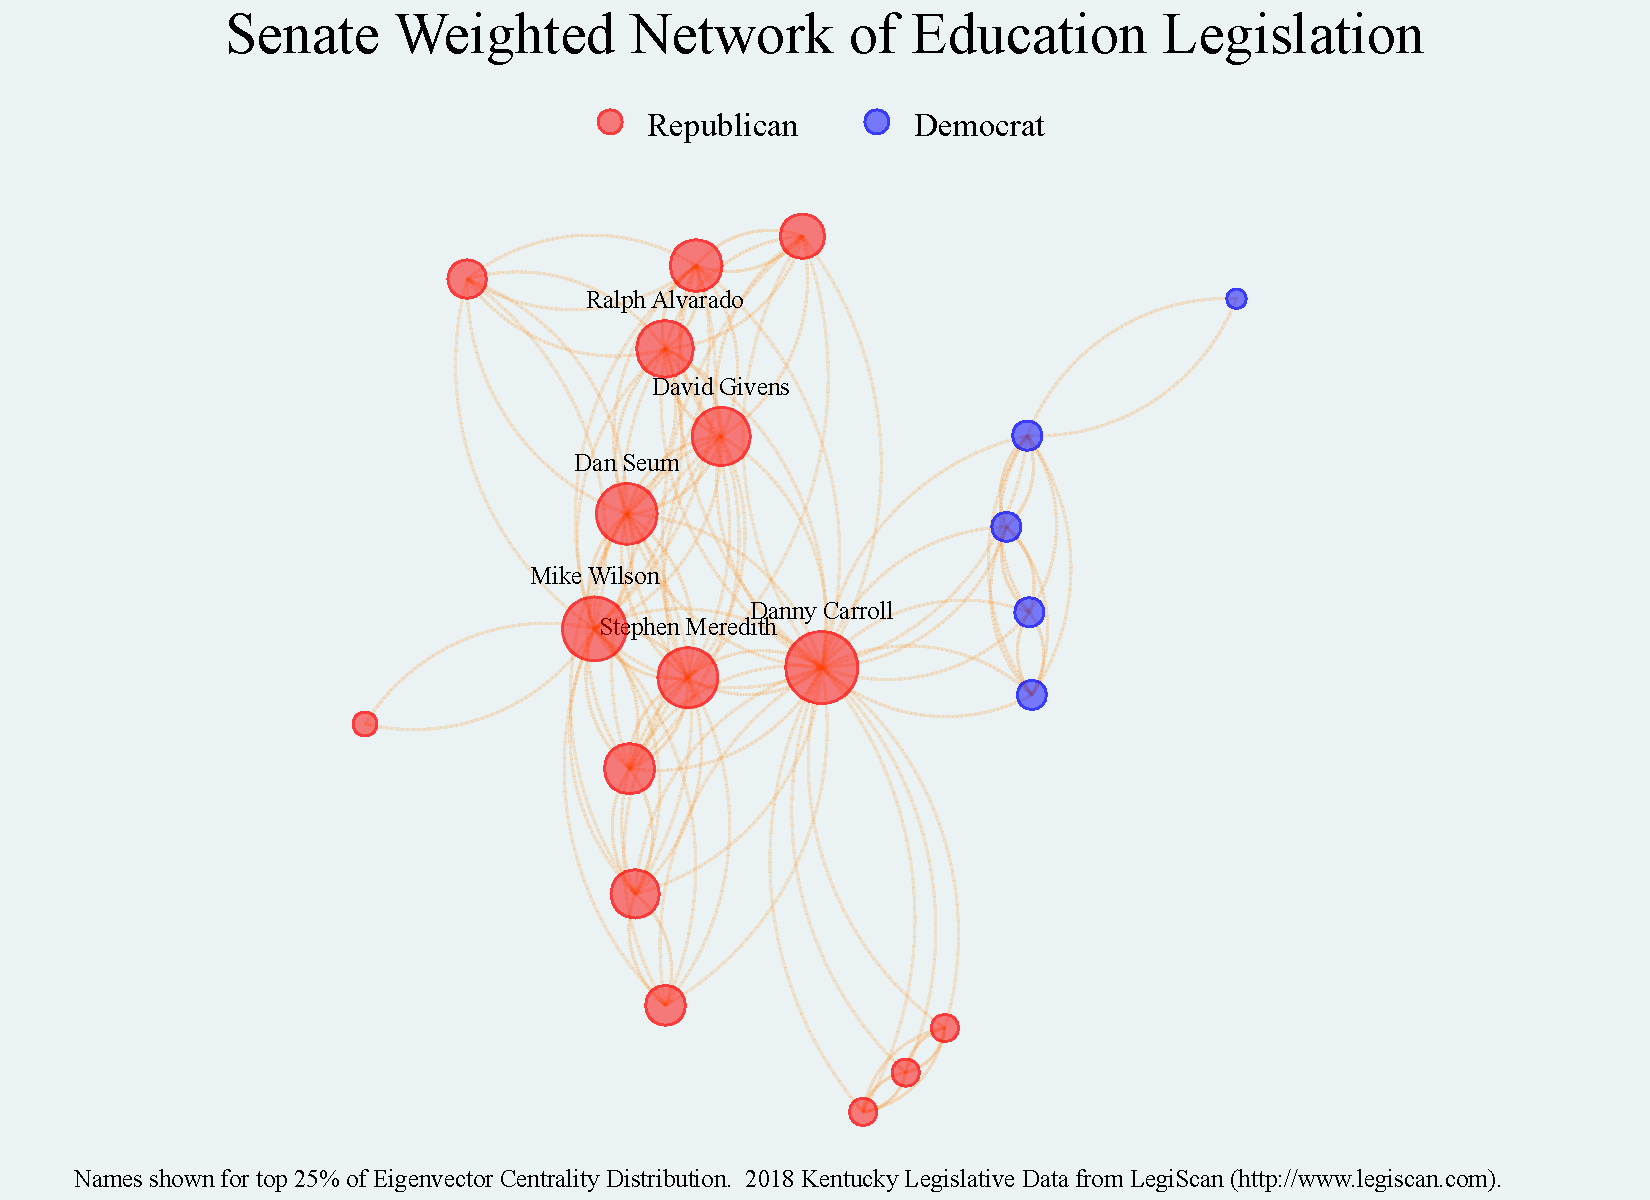
\includegraphics[scale=0.95]{senateedwgt-graph.pdf}
							\caption{Senate ECN \label{senateed}}
						\end{figure}
					\end{column} % End of column 2.1
					\begin{column}{\onecolwid}\vspace{-.6in} % The second column within column 2 (column 2.2)
						\begin{figure}
							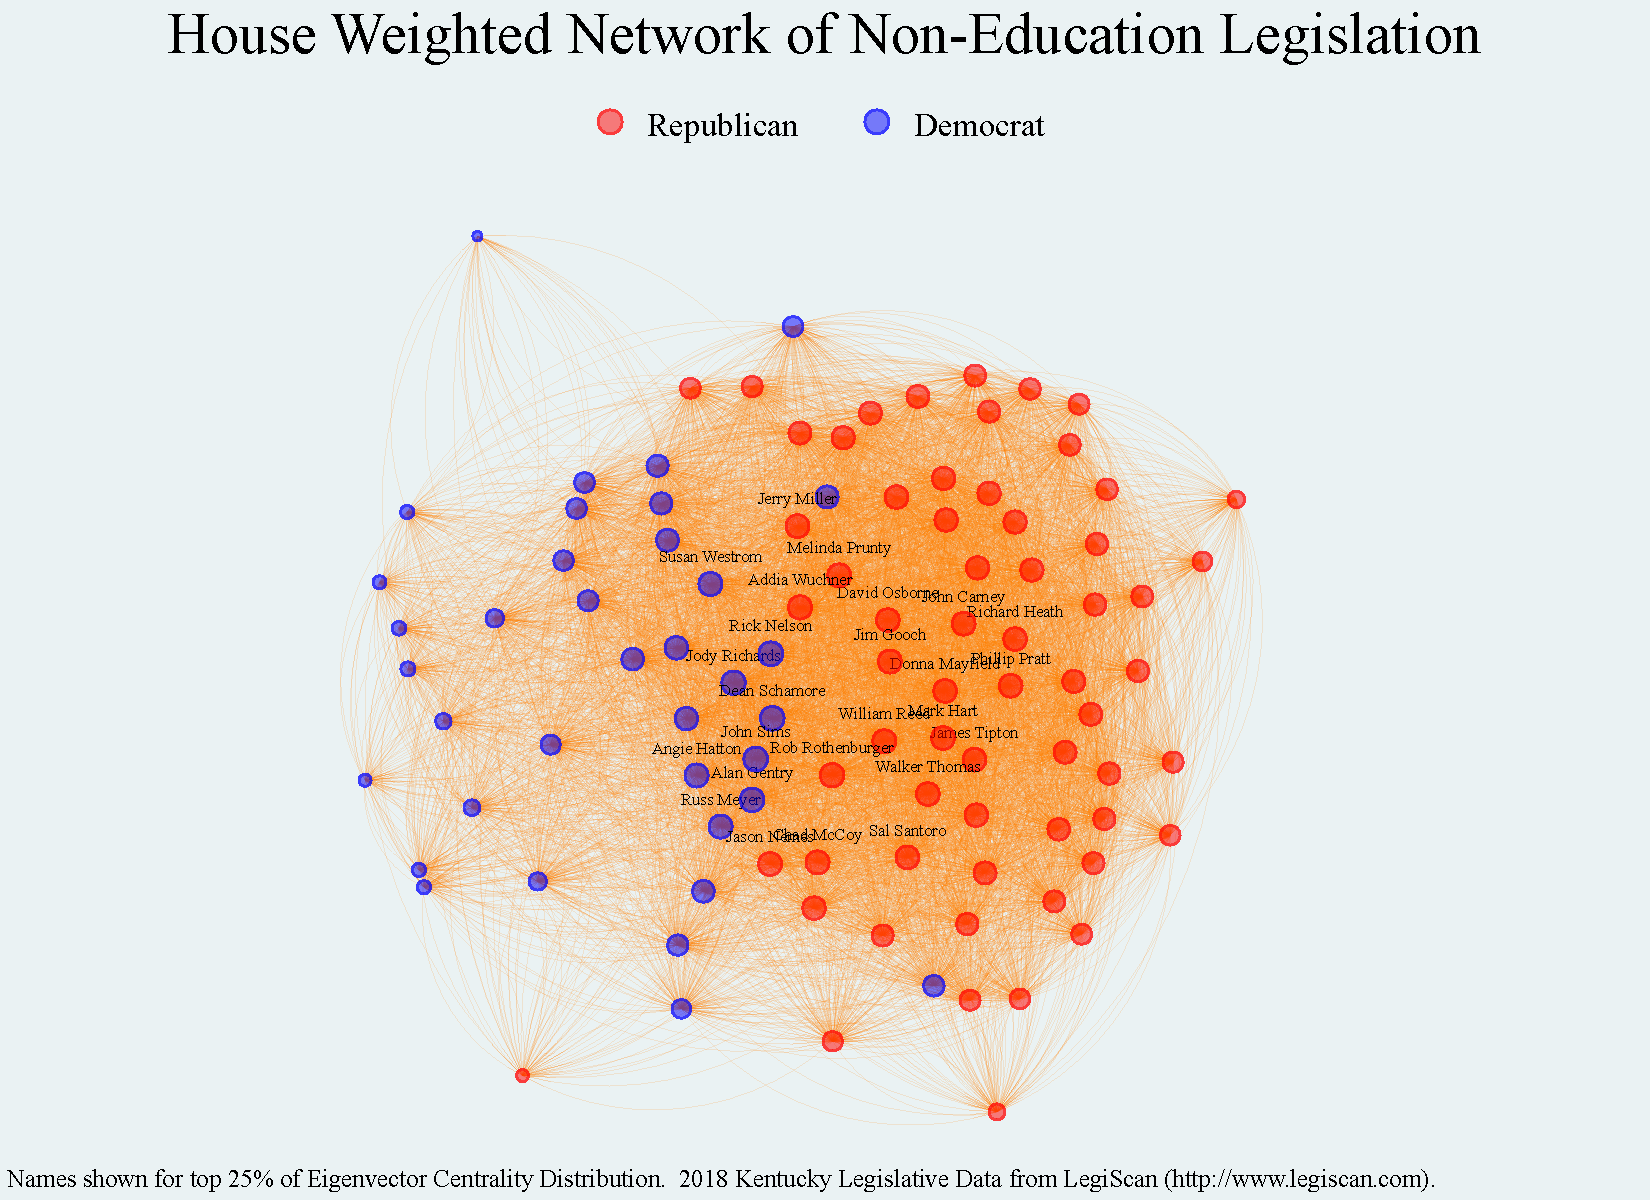
\includegraphics[scale=0.95]{housenonedwgt-graph.pdf}
							\caption{House NECN \label{housenoned}}
						\end{figure}
					\end{column} % End of column 2.2
				\end{columns} % End of the split of column 2 - any content after this will now take up 2 columns width
				\begin{block}{Data}
					Data for Kentucky's 2018 regular session were retrieved from \textcite{legiscan2018} 
					\url{(http://www.legiscan.com)}.  We used regular expressions to identify education related 
					legislation and to identify legislation from resolutions and chamber rules. \\
					Once the data were assembled into an edgelist formatted data structure, we used commands 
					from the \texttt{nwcommands} package \parencite{grund2015} to construct the NECN and ECN networks 
					for the house and senate. 
				\end{block}
				\begin{block}{Methods}
					We chose to focus on weighted networks in our analysis assuming that legislators who
					co-sponsor more legislation would be more influential and better reflects the social ties
					that exist between legislators co-sponsoring each others' bills \parencite{hangal2010}.  
					Additionally, we selected the Eigenvector centrality measure to identify influence that
					each legislator has across the entire network \parencite{landherr2010}.  
				\end{block}
				
				\begin{alertblock}{Results}
					The graphs above provide visual representations of the cosponsorship networks across chambers and legislation type.  
					Only legislators with Eigenvector centrality scores greater than or equal to the 75\textsuperscript{th} percentile 
					or higher are identified in the visualiations. \\ 
					\vspace{0.5cm}
					In figure \ref{senatenoned} none of the senators holding leadership positions are identified as highly influential in the NECN.  	
					The majority whip (Mike Wilson) does appear to be an influential actor in the senate's ECN (figure \ref{senateed}).  
					However, neither the chair or the vice chair of the senate's education committee appear to be empirically influential in either 
					the NECN or ECN. \\
					\vspace{0.5cm}
					Unlike the senate, some house members in leadership positions do appear to be highly influential in the NECN 
					(figure \ref{housenoned}). 	More specifically, the house speaker pro-tempore and the chair of the house's education
					committee, David Osborne and John Carney respectively, appear to be influential in the broader legislative context 
					of the house.  In the context of education legislation in the house, the only house member in a leadership position
					to be empirically identified as influential is the education committee chair, John Carney (see figure \ref{houseed}). \\
					\begin{table}
						\caption{\textit{Correlations Between Networks and Political Party.} \label{results}}
						\begin{tabular}{l l l l l}
							\toprule
							\textbf{Chamber} & \textbf{Network} & \textbf{Network/Covariate} & \textbf{$\rho$} & \textbf{p-value} \\ 
							\midrule
							House & Education & Non-Education & 0.38 & 0.0 \\
							House & Non-Education & Political Party & 0.42 & 0.0 \\
							House & Education & Political Party & 0.06 & 0.014 \\
							Senate & Education & Non-Education & 0.46 & 0.0 \\
							Senate & Non-Education & Political Party & 0.23 & 0.002 \\
							Senate & Education & Political Party & 0.21 & 0.0 \\
							\bottomrule
						\end{tabular}
					\end{table}
					Although there are moderate correlations between the NECN and ECN in each chamber (see table \ref{results}), there 
					are differences in the actors wielding the most influence between those networks. More importantly, the correlations
					between political party affiliation and cosponsorship networks may be an indicator of the partisan nature of the 
					legislature in the Commonwealth of Kentucky.

				\end{alertblock} 

			\end{column} % End of the second column

			\begin{column}{\sepwid}\end{column} % Empty spacer column
			
			\begin{column}{\onecolwid} % The third column
				%----------------------------------------------------------------------------------------
				%	CONCLUSION
				%----------------------------------------------------------------------------------------
				\begin{figure}
					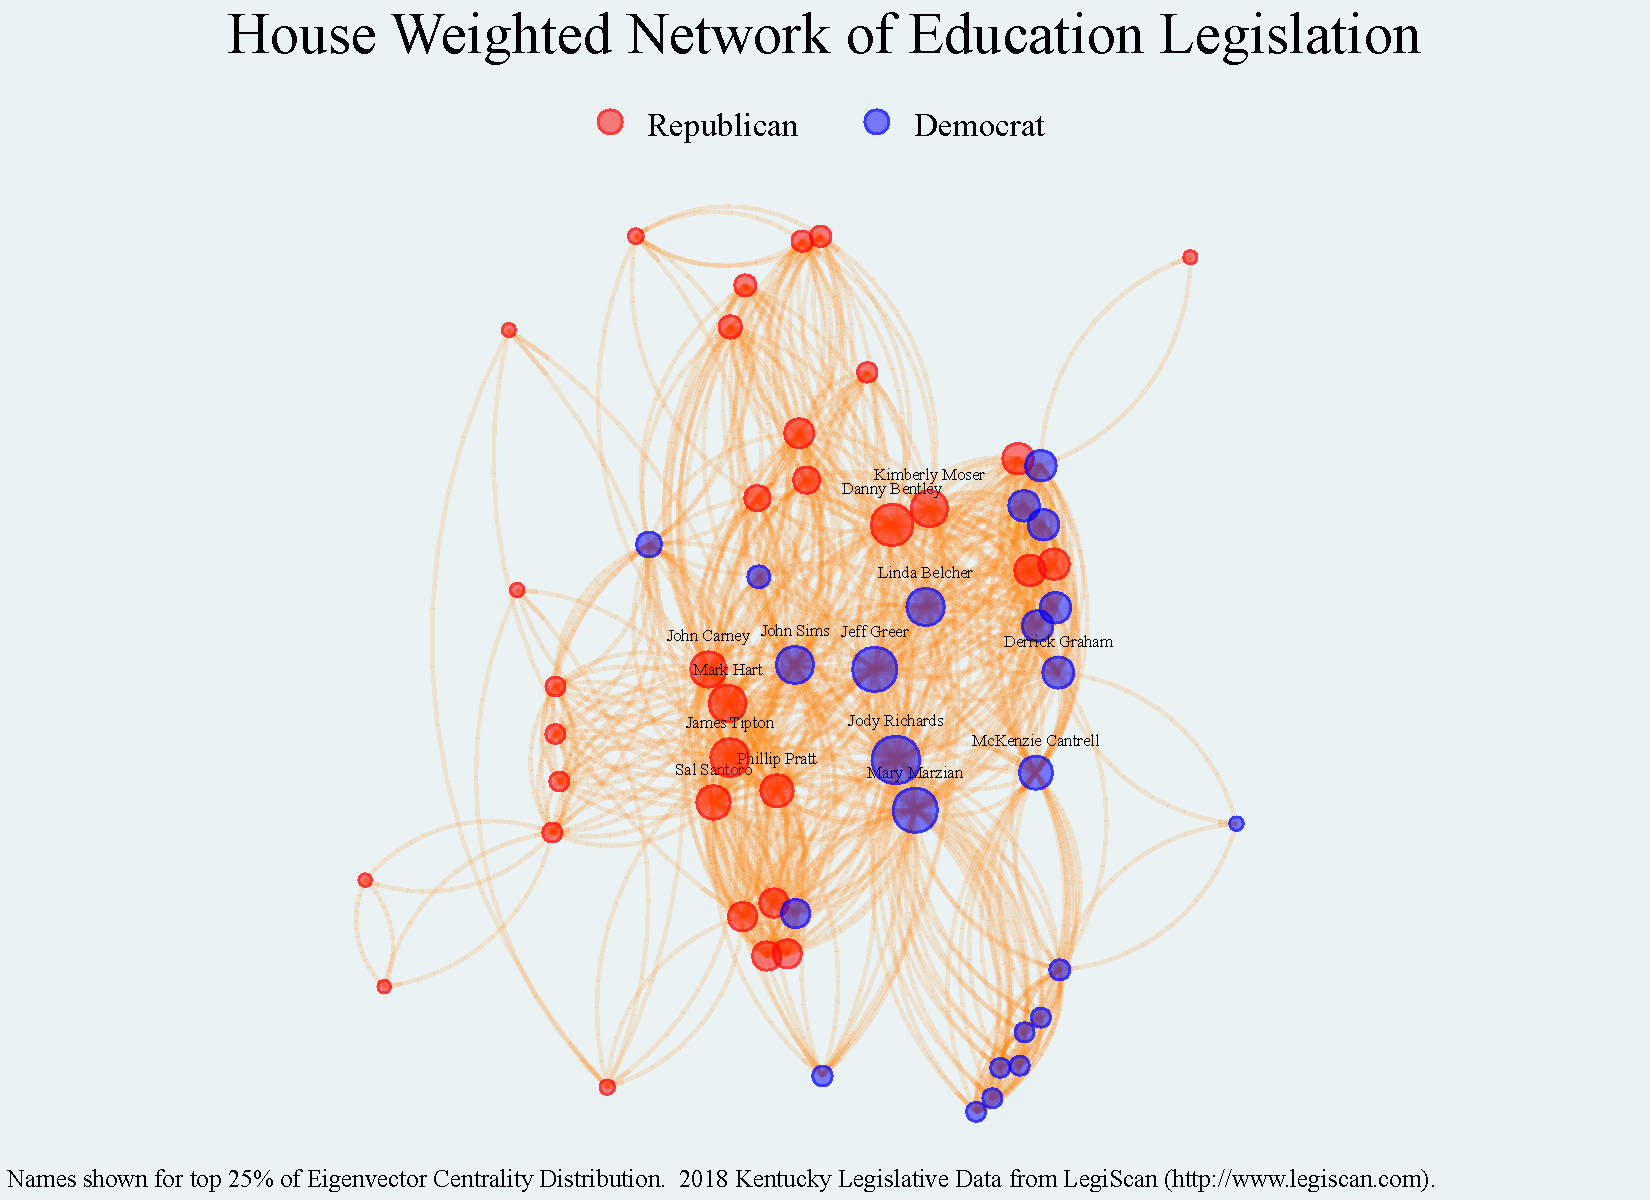
\includegraphics[scale=0.95]{houseedwgt-graph.pdf}
					\caption{House ECN \label{houseed}}
				\end{figure}
%				\begin{block}{Discussion}
%				\end{block}
				\begin{block}{Conclusion}
					While the estimated correlations in the cosponsorship networks are generally on the smaller side, there do appear 
					to be some notable indicators of partisanship.  For example, there appears to be almost no relationship between 
					political party affiliation and the ECN in the house (table \ref{results}), while the correlation between the 
					NECN and ECN in the Senate do not vary much.  Most importantly, we find it interesting the legislative leaders 
					do not appear to be highly influential in the context of cosponsoring of legislation.  We believe a better 
					understanding of cosponsorship networks and networks related to voting outcomes could provide a more effective means 
					for educational organizations to deploy resources to more effectively advocate for educational policy changes and reforms.
				\end{block}
				%----------------------------------------------------------------------------------------
				%	REFERENCES
				%----------------------------------------------------------------------------------------
				\begin{block}{References}
					\nocite{*}  % Insert publications even if they are not cited in the poster
					\small{\printbibliography}
				\end{block}
				%----------------------------------------------------------------------------------------
				%	ACKNOWLEDGEMENTS
				%----------------------------------------------------------------------------------------
				% \setbeamercolor{block title}{fg=red,bg=white} % Change the block title color
				% \begin{block}{Acknowledgements}
				% 	\small{\rmfamily{Nam mollis tristique neque eu luctus. Suspendisse rutrum congue 
				% 	nisi sed convallis. Aenean id neque dolor. Pellentesque habitant morbi tristique 
				% 	senectus et netus et malesuada fames ac turpis egestas.}} \\
				% \end{block}
				%----------------------------------------------------------------------------------------
				%	CONTACT INFORMATION
				%----------------------------------------------------------------------------------------
				\setbeamercolor{block alerted title}{fg=black,bg=norange} % Change the alert block title colors
				\setbeamercolor{block alerted body}{fg=black,bg=white} % Change the alert block body colors
				\begin{alertblock}{Contact Information}
					\begin{itemize}
						\item Web: \href{https://github.com/rdelcampo}{https://github.com/rdelcampo}
						\item Email: \href{mailto:roxanadelcampo@gmail.com}{rdcampo@uw.edu}
					\end{itemize}
				\end{alertblock}
			\end{column} % End of the third column
		\end{columns} % End of all the columns in the poster
	\end{frame} % End of the enclosing frame
\end{document}
